% Chapter 6
\chapter{Multispectral Human Skin Detection}% Main chapter title

\label{Chapter6} % For referencing the chapter elsewhere, use \ref{Chapter1}

\lhead{Chapter 6. \emph{Multispectral}} % This is for the header on each page - perhaps a shortened title

%----------------------------------------------------------------------------------------
\section{Introduction}
The conventional methods for detecting objects, which employ pattern
recognition, have many problems, for example, an increase in processing time, 
a difficulty of detecting occluded objects, a necessity of huge data for machine
learning and so on. To overcome these problems, a method for detecting human skin 
that employs a spectroscopic camera will be studied. Each substance has its
own reflection characteristics. In particular, human
skin reflects flesh-colored light in the visible region and
absorbs light with a wavelength of 970 nm. Thus, to detect human skin, 
a multi-band camera that has red, green, blue, 870, 970, and 1050 nm filters will be
studied. By using this multi-band camera, human
skin in Y Cr Cb color space around the visible region
and dips around 970 nm in the near-infrared region is detected.\cite{Kanzawa_humanskin}

\begin{figure}[ht]
  \label{fig:chap6-Reflectance}
  \centering
	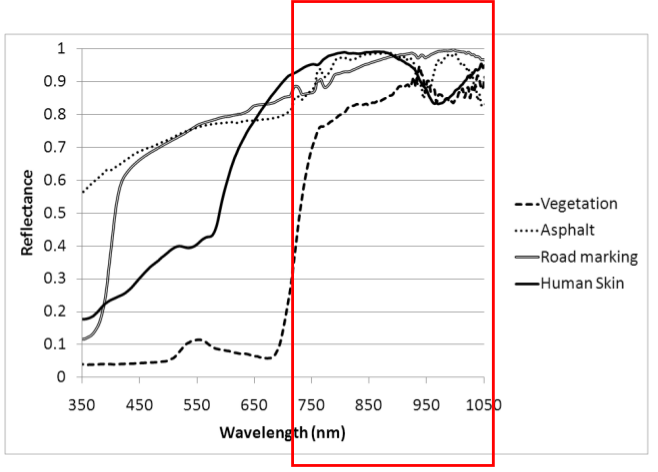
\includegraphics[width=0.7\textwidth, keepaspectratio=true]{chap6-Reflectance.png}
	\caption{Reflectance spectra of various substances.}
\end{figure}

\section {Reflectance Spectrum of Human Skin}
Spectroscopy is the study of how substances absorb,
transmit, or reflect light. A conventional camera sensor
can obtain images in the ultraviolet (UV),
Vis, and NIR regions. UV–Vis–NIR spectroscopy is
applied for optical absorbance and reflectance measurements in the wavelength 
range 200–1500 nm. Because a substance has its own unique reflectance 
characteristics, we can distinguish a substance by analyzing the
light reflectance. Reflectance spectra of some substances, for example
asphalt, road markings and human skin are depicted in \autoref {fig:chap6-Reflectance}. 
The horizontal and vertical axis show the wavelength and reflectance, respectively.

\autoref{fig:chap6-humanskin} shows only a reflectance spectrum of human
skin. Skin has a lower reflectance at shorter wavelengths (about 350 nm) than at 
longer wavelengths (about 1050 nm). In particular, skin has a unique
property that it absorbs light around a wavelength of 970nm in the NIR region. 
\begin{figure}[ht]
  \label{fig:chap6-humanskin}
  \centering
	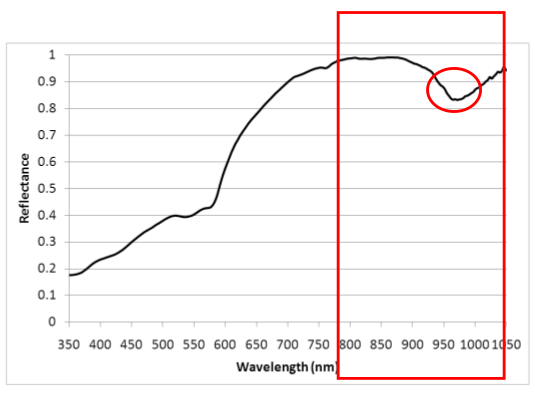
\includegraphics[width=0.7\textwidth, keepaspectratio=true]{chap6-humanskin.png}
	\caption{Reflectance spectra of human skin.}
\end{figure}

The reflectance spectra of skin from about 50 people who have various
races are measured; all the spectra revealed that light was absorbed
at a wavelength of 970 nm, as shown in \autoref {fig:chap6-humanrace}.

\begin{figure}[h]
  \label{fig:chap6-humanrace}
  \centering
	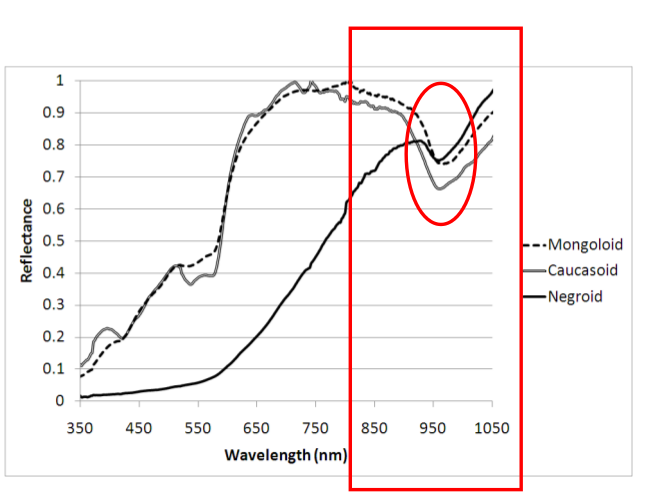
\includegraphics[width=0.7\textwidth, keepaspectratio=true]{chap6-humanrace.png}
	\caption{Spectra of various human skin.}
\end{figure}

%----------------------------------------------------------------------------------------
\section{Multi-Camera Module}
Human skin reflects flesh-colored light in the Vis region and absorbs light 
with a wavelength of 970 nm in the NIR region. A multi-band camera is studied to
exploit these characteristics. It has two types of cameras: a Vis camera that 
acquires three images around Vis regions as a conventional color camera and 
a NIR camera that can acquire three images in individual NIR wavelengths (870, 950,
1050nm). \autoref{fig:chap6-mcam} shows a photograph of the multi-band camera schematic.

\begin{figure}[hb]
  \label{fig:chap6-mcam}
  \centering
	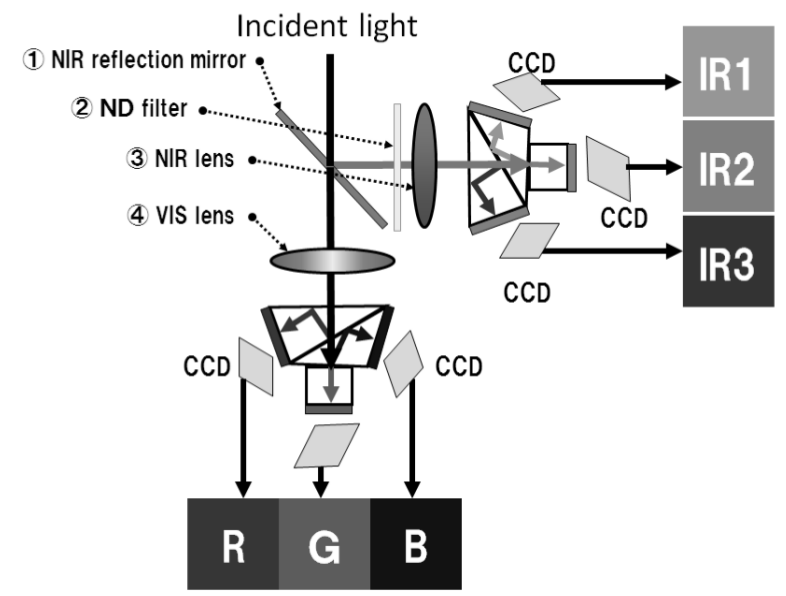
\includegraphics[width=0.7\textwidth, keepaspectratio=true]{chap6-mcam.png}
	\caption{Schematic diagram of the multi-camera module.}
\end{figure}

\section {Human Skin Detection}
Conventionally, for detecting human skin from images, 
visible color image processing methods are used.
However, it has been well known that color information is easily affected 
from a change of illumination condition. A NIR image processing method is proposed 
to detect human skin. This method is based on the characteristics of spectroscopy
around NIR region, therefore unaffected from visible
light. But, since clouds and water vapor absorbs light
with a wavelength of 940nm as shown in \autoref {fig:chap6-water}, 
it is difficult to distinguish human skin, which absorbs light with a wavelength 
of 970nm, from clouds. To overcome above problems, a multi-band camera is studied.
Both visible color and NIR image processing methods are combined for detecting 
human skin.

\begin{figure}[hb]
  \label{fig:chap6-water}
  \centering
	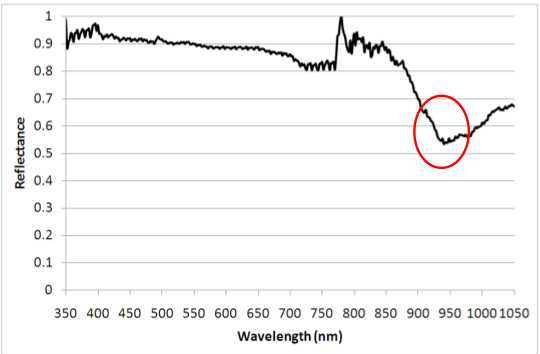
\includegraphics[width=0.7\textwidth, keepaspectratio=true]{chap6-water.png}
	\caption{Reflectance spectra of clouds and water vapor.}
\end{figure}
